\documentclass[11pt]{article}

\usepackage{amsmath}
\usepackage[a4paper, margin=0.5in]{geometry}
\usepackage{graphicx} % daj an 1in jak chcesz normalniejszy margines, ale kod mi się w linii nie mieści :P
\usepackage[utf8]{inputenc}
\usepackage[T1]{fontenc}
\usepackage[polish]{babel}
\usepackage{float}
\usepackage{hyperref}
\usepackage{cleveref}
\usepackage{subfigure}
\usepackage{multirow}

\title{Zadanie 3. Wykorzystanie ocen ruchów z poprzednich iteracji i ruchów
kandydackich w lokalnym przeszukiwaniu}
\author{Oskar Kiliańczyk 151863 \& Wojciech Kot 151879}
\date{}

\begin{document}

\maketitle
\newpage

\section{Opis zadania}\label{sec:opis-zadania}

Celem eksperymentu jest poprawa efektywności czasowej lokalnego przeszukiwania w wersji stromej, wykorzystującego najlepsze sąsiedztwo z poprzedniego zadania.
Porównujemy wersję bazową z dwiema modyfikacjami: uporządkowaną listą ruchów oraz ruchem kandydackim.
Każdy algorytm uruchamiany jest 100 razy na każdej instancji, startując z losowych rozwiązań.
Dla porównania uwzględniamy również najlepszą heurystykę konstrukcyjną z zadania 1.

\section{Opisy algorytmów}\label{sec:opisy-alg}

\subsection{Te same co w poprzednich sprawozdaniach}\label{subsec:te-same-co-w-poprzednich-sprawozdaniach}

\subsubsection{Steepest}\label{subsec:steepest}

\begin{enumerate}
  \item Dopóki możliwa jest poprawa:
  \begin{enumerate}
    \item Przeszukaj wszystkie możliwe modyfikacje ścieżek:
    \begin{itemize}
      \item zmiany lokalne w jednej ścieżce (zamiana dwóch wierzchołków lub odwrócenie fragmentu),
      \item wymiany wierzchołków między ścieżkami.
    \end{itemize}
    \item Wybierz modyfikację dającą największą poprawę.
    \item Wprowadź ją do odpowiedniej ścieżki lub ścieżek.
  \end{enumerate}
  \item Zwróć ulepszone ścieżki.
\end{enumerate}


\subsubsection{Nasz własny algorytm}\label{subsec:nasz-wasny-algorytm}

Nasza heurystyka konstrukcyjna cechuje się podejściem zachłannym, ale wykorzystuje pewną wiedzę dziedzinową,
a mianowicie to, że znacznie lepsze wyniki da się uzyskać kiedy wpierw dobierze się mądry podział wierzchołków startowych.

\begin{enumerate}
    \item Utworzenie listy pozostałych wierzchołków (wszystkie możliwe, poza startowymi)
    \item Utworzenie dwóch list zawierających odpowiednio dystanse każdego wierzchołka do pierwszego i do drugiego wierzchołka startowego
    \item Sortowanie utworzonych uprzednio list dystansów wierzchołków
    \item Aż do przydzielenia wszystkich wierzchołków z listy pozostałych wierzchołków wykonuje:
    \item Zmianę decyzji do którego zestawu wierzchołków obecnie będzie przydzielać wierzchołek (aby robić to naprzemiennie)
    \item Wyszukuje pierwszy wierzchołek na liście dystansów który nie został jeszcze przydzielony do żadnego zestawu i przydziela go tam
\end{enumerate}

W skutek zastosowania takiego przydziału uzyskujemy dwa równo-liczne zbiory, oraz zapewniamy że gdyby ilość badanych wierzchołków była nieparzysta, to zbiory będą różnić się długością najwyżej o 1.

Następnie wykorzystujemy tradycyjny algorytm rozbudowy cyklu w oparciu o dwużal, osobno na obu listach.
Wygląda on następująco:

\begin{enumerate}
    \item Algorytm zaczyna od ścieżki zawierającej wierzchołek startowy podwójnie
    \item Dopóki w ścieżce nie znajdują sie wszystkie wierzchołki z zadanego mu zestawu powtarza:
    \item Dla każdego nieodwiedzonego wierzchołka oblicza koszty jego wstawienia
    \item Następnie oblicza żal (dwużal) dla danego wierzchołka
    \item Rozbudowuje cykl o wierzchołek z największym obliczonym żalem i zaznacza go jako odwiedzonego
    \item Zwraca ścieżkę
\end{enumerate}

Używając takiej funkcji osobno na obu zbiorach wierzchołków uzyskujemy dwie ścieżki i zwracamy do programu głównego.

% todo opisy
% todo pseudokody

\section{Wyniki}\label{sec:wyniki}

\subsection{Tabela wynikowa}\label{subsec:tabela-wynikowa}

\begin{table}[ht]
\centering
\resizebox{\textwidth}{!}{
\begin{tabular}{|c||c|c|c||c|c|c||c|c|}
\hline
\textbf{Algorytm} & \textbf{Best} & \textbf{Avg} & \textbf{Worst} & \textbf{Best Time} & \textbf{Avg Time} & \textbf{Worst Time} & \textbf{Best Diff} & \textbf{Avg Diff} \\
\hline
\texttt{split\_paths\_regret\_TSP} & 30426 & 32893 & 36854 & 0.0943059 & 0.105313 & 0.206992 & & \\
\hline
\texttt{traverse\_steepest\_edge} & 35949 & 38818.8 & 41812 & 3.70818 & 4.1397 & 4.53379 & 325405 & 301537 \\
\hline
\texttt{steepest\_LM} & 34643 & 38673 & 41570 & 1.02937 & 1.30407 & 1.92433 & 327271 & 301518 \\
\hline
\texttt{steepest\_kandydackie} & 36656 & 39723.4 & 43659 & 0.889616 & 1.04703 & 1.90562 & 323577 & 298848 \\
\hline
\end{tabular}
}
\caption{Wyniki dla \texttt{kroA200}}
\end{table}

\begin{table}[ht]
\centering
\resizebox{\textwidth}{!}{
\begin{tabular}{|c||c|c|c||c|c|c||c|c|}
\hline
\textbf{Algorytm} & \textbf{Best} & \textbf{Avg} & \textbf{Worst} & \textbf{Best Time} & \textbf{Avg Time} & \textbf{Worst Time} & \textbf{Best Diff} & \textbf{Avg Diff} \\
\hline
\texttt{split\_paths\_regret\_TSP} & 31218 & 33102.7 & 36913 & 0.0939048 & 0.0999451 & 0.131889 & & \\
\hline
\texttt{traverse\_steepest\_edge} & 36556 & 38791.3 & 41839 & 3.94789 & 4.60979 & 6.5536 & 329070 & 293891 \\
\hline
\texttt{steepest\_LM} & 36309 & 38794.7 & 41938 & 0.97498 & 1.25639 & 1.55901 & 322191 & 293913 \\
\hline
\texttt{steepest\_kandydackie} & 37372 & 39808.4 & 41720 & 0.861845 & 0.965179 & 1.08236 & 325756 & 292558 \\
\hline
\end{tabular}
}
\caption{Wyniki dla \texttt{kroB200}}
\end{table}



\subsection{Wizualizacja wyników}\label{subsec:wizualizacja-wynikow}

\subsubsection{Algorytm stromy, bazowy}\label{subsubsec:algorytm-stromy-bazowy}

\begin{figure}[H]
    \begin{minipage}[t]{0.45\textwidth}
        \centering
        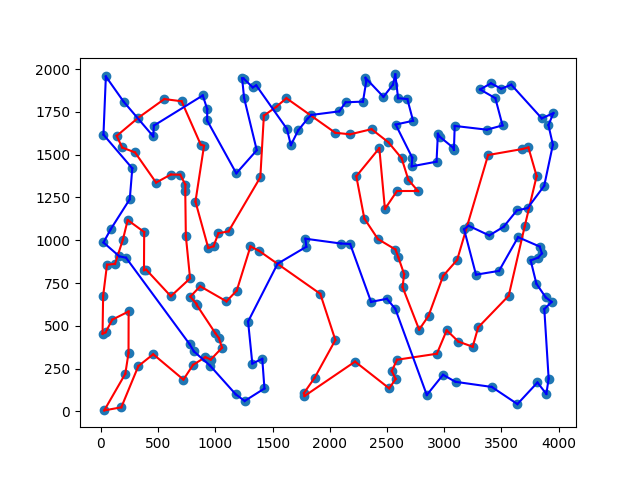
\includegraphics[width=\linewidth]{best_paths/kroA200/traverse_steepest_edge}
        \caption{kroA200, losowy start}
    \end{minipage}
    \hfill
    \begin{minipage}[t]{0.45\textwidth}
        \centering
        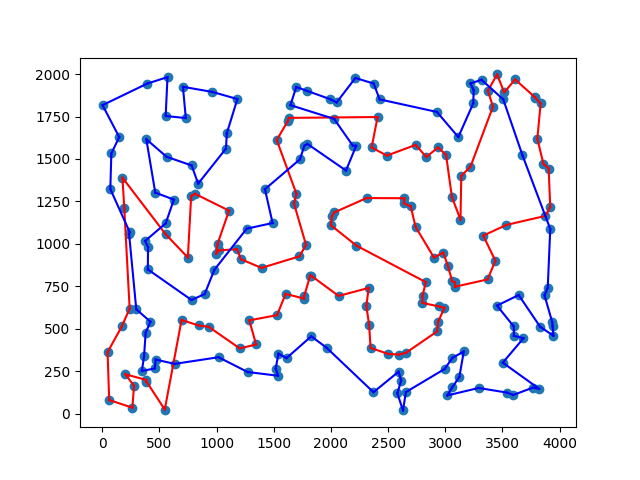
\includegraphics[width=\linewidth]{best_paths/kroB200/traverse_steepest_edge}
        \caption{kroB200, losowy start}
    \end{minipage}\label{fig:figure1}
\end{figure}


\subsubsection{Algorytm stromy z listą ruchów}\label{subsubsec:algorytm-stromy-z-lista-ruchow}

\begin{figure}[H]
    \begin{minipage}[t]{0.45\textwidth}
        \centering
        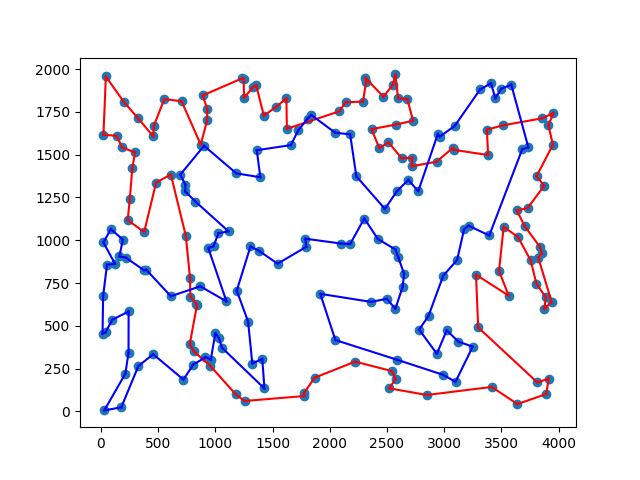
\includegraphics[width=\linewidth]{best_paths/kroA200/steepest_LM}
        \caption{kroA200, losowy start}
    \end{minipage}
    \hfill
    \begin{minipage}[t]{0.45\textwidth}
        \centering
        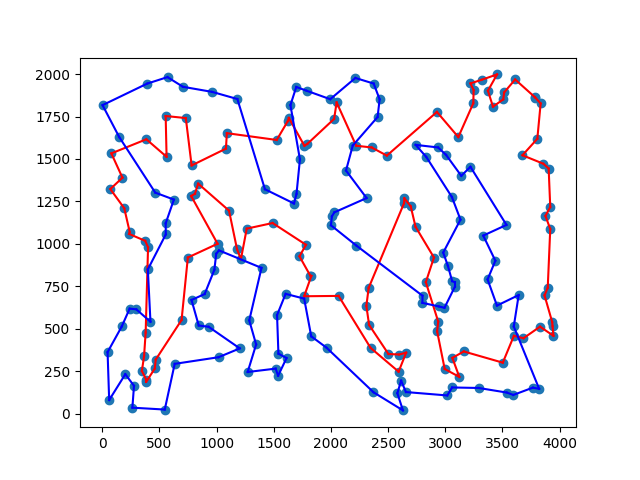
\includegraphics[width=\linewidth]{best_paths/kroB200/steepest_LM}
        \caption{kroB200, losowy start}
    \end{minipage}\label{fig:figure2}
\end{figure}


\subsubsection{Algorytm stromy z mechanizmem ruchów kandydackich}\label{subsubsec:algorytm-stromy-z-mechanizmem-ruchow-kandydackich}

\begin{figure}[H]
    \begin{minipage}[t]{0.45\textwidth}
        \centering
        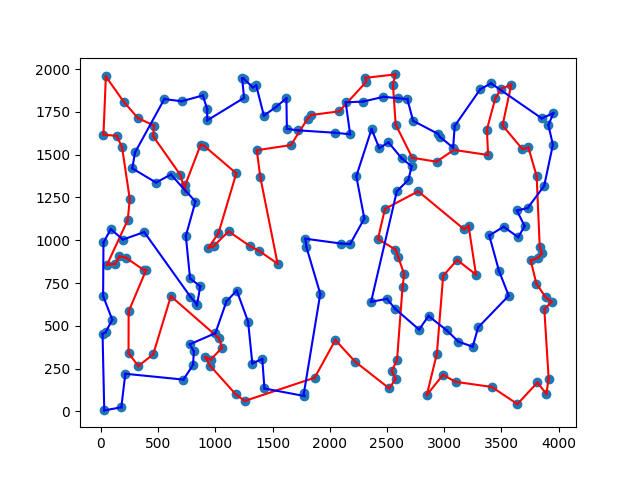
\includegraphics[width=\linewidth]{best_paths/kroA200/steepest_kandydackie}
        \caption{kroA200, losowy start}
    \end{minipage}
    \hfill
    \begin{minipage}[t]{0.45\textwidth}
        \centering
        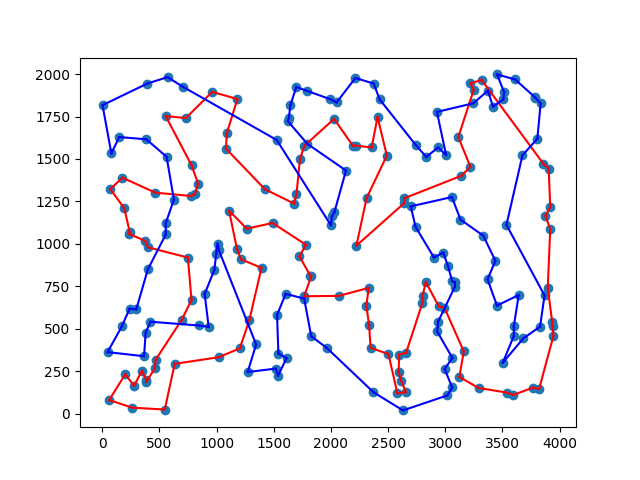
\includegraphics[width=\linewidth]{best_paths/kroB200/steepest_kandydackie}
        \caption{kroB200, losowy start}
    \end{minipage}\label{fig:figure3}
\end{figure}


\subsubsection{Heurystyka konstrukcyjna}\label{subsubsec:heurystyka-konstrukcyjna}

\begin{figure}[H]
    \begin{minipage}[t]{0.45\textwidth}
        \centering
        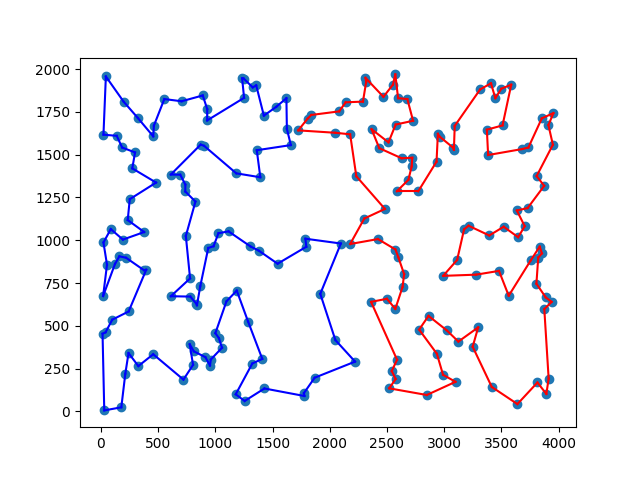
\includegraphics[width=\linewidth]{best_paths/kroA200/split_paths_regret_TSP}
        \caption{kroA200, losowy start}
    \end{minipage}
    \hfill
    \begin{minipage}[t]{0.45\textwidth}
        \centering
        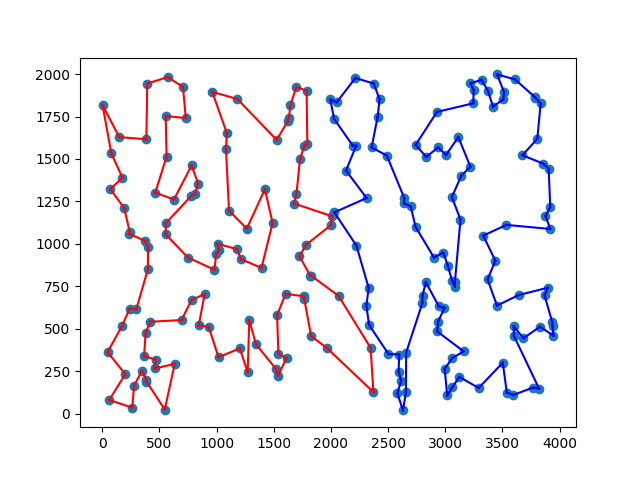
\includegraphics[width=\linewidth]{best_paths/kroB200/split_paths_regret_TSP}
        \caption{kroB200, losowy start}
    \end{minipage}\label{fig:figure4}
\end{figure}


\section{Wnioski i analiza wyników}\label{sec:wnioski}

Na podstawie wyników można zauważyć, że algorytm stromy z listą ruchów oraz algorytm stromy z mechanizmem ruchów kandydackich są znacznie bardziej efektywne niż algorytm bazowy.
W przypadku instancji kroA200 algorytm stromy z listą ruchów osiągnął lepszy wynik, natomiast w przypadku instancji kroB200 algorytm stromy z mechanizmem ruchów kandydackich okazał się lepszy.
Niezależnie od instancji algorytm korzystający z ruchów kandydackich okazał się odrobinę bardziej efektywny czasowo.
Wyniki naszej heurystyki konstrukcyjnej są wciąż najlepsze, jednak jest to przede wszystkim zasługa dobrego startowego podziału, czyli zastosowania swego rodzaju wiedzy dziedzinowej,
a to sugeruje, że algorytmy lokalnego przeszukiwania mogą być użyte do poprawy wyników heurystyki konstrukcyjnej, ale nie jako osobna metoda znajdowania optimum rozpoczynając z rozwiązań losowych.
Poprzednie zadanie pokazało, że algorytmy lokalnego przeszukiwania są bardziej efektywne w przypadku, gdy startujemy z rozwiązań konstrukcyjnych.


\section{Link do repozytorium}\label{sec:link-do-repo}
Kod źródłowy w repozytorium GitHub dostępny pod linkiem: \\
\href{https://github.com/KotZPolibudy/PUT_IMO/tree/main/Lab3%20-%20Local_augmented}{Repozytorium}.

\end{document}
